\documentclass[conference]{IEEEtran}
\IEEEoverridecommandlockouts

\usepackage[T1]{fontenc}
\usepackage{cite}
\usepackage{amsmath,amssymb,amsfonts}
\usepackage{graphicx}
\usepackage{textcomp}
\usepackage{xcolor}
\usepackage{listings}
\usepackage{tikz}
\usepackage{framed}

\lstset{
    language=Verilog,
    %basicstyle=\ttfamily\scriptsize,
    basicstyle=\ttfamily\footnotesize,
    keywordstyle=\color{blue},
    commentstyle=\color{green!50!black}\tiny,
    stringstyle=\color{red},
    backgroundcolor=\color{green!10},
    showstringspaces=false,
    numbers=left,
    numberstyle=\tiny\color{gray},
    frame=single,
    breaklines=true,
    tabsize=4,
    columns=flexible, % 灵活列宽
    breaklines=false, % 不自动换行
    aboveskip=0pt, % 减少上方间距
    belowskip=0pt, % 减少下方间距
    captionpos=b
}


\definecolor{eclipseStrings}{RGB}{42,0.0,255}
\definecolor{eclipseKeywords}{RGB}{127,0,85}
\definecolor{darkgray}{rgb}{0.4, 0.4, 0.4}

% 手动定义 JSON 语言规则
\lstdefinelanguage{json}{
    basicstyle=\normalfont\ttfamily\scriptsize,
    showstringspaces=false,
    breaklines=true,
    morestring=[b]", % 识别双引号里的字符串
    stringstyle=\color{eclipseStrings}, % 字符串颜色
    morecomment=[s]{/*}{*/},
    morecomment=[l]//,
    keywordstyle=\color{eclipseKeywords}\bfseries,
    ndkeywordstyle=\color{darkgray}\bfseries,
}

\usetikzlibrary{arrows.meta,positioning,fit,calc,backgrounds,shapes}

%\lstset{
%    language=Verilog,
%    basicstyle=\ttfamily\footnotesize,
%    keywordstyle=\color{blue},
%    commentstyle=\color{green!40!black},
%    stringstyle=\color{red!70!black},
%    showstringspaces=false,
%    frame=single,
%    breaklines=true,
%    columns=fullflexible
%}

\def\BibTeX{{\rm B\kern-.05em{\sc i\kern-.025em b}\kern-.08em
    T\kern-.1667em\lower.7ex\hbox{E}\kern-.125emX}}

\begin{document}

\title{MileSE: Milestone-Guided Symbolic Execution for Multi-Cycle RTL Verification}

\IEEEspecialpapernotice{\vspace{-2em}}
%\author{
%Jiahui Liang$^{1,2}$, Qiusong Yang$^{1,2*}$, Yiwei Ci$^{1,2}$ \\
%$^{1}$Institute of Software, Chinese Academy of Sciences, Beijing, China \\
%$^{2}$University of Chinese Academy of Sciences, Beijing, China \\
%*Corresponding Author: qiusong@iscas.ac.cn
%}
\IEEEaftertitletext{}

\maketitle

\begin{abstract}
Symbolic execution (SE) is a rigorous method for finding deep hardware vulnerabilities. However, applying SE to multi-cycle Register-Transfer Level (RTL) designs often leads to severe temporal path explosion. While traditional undirected search strategies are sound, they typically demand substantial computational resources on irrelevant states. Conversely, Large Language Models (LLMs) can provide promising heuristic guidance but suffer from unreliability due to hallucinations.

This paper introduces MileSE, a milestone-guided symbolic execution framework designed for multi-cycle RTL verification to effectively reach deep sequential targets. MileSE leverages LLM-generated milestones to dynamically prioritize path exploration. To mitigate LLM hallucinations and temporal mismatches, our framework incorporates system-level fault-tolerance mechanisms, including sliding-window lookahead and bounded pruning, which reduce the calling of the solvers. Experimental results demonstrate that our approach can find more bugs and dramatically reduces verification overhead (e.g., time, memory, and SMT queries) , outperforming state-of-the-art techniques.
\end{abstract}

\begin{IEEEkeywords}
Symbolic Execution, RTL Verification, Hardware Security, Directed Search, Large Language Models
\end{IEEEkeywords}

\section{Introduction}
\label{sec:intro}

The complexity of hardware designs has shifted the burden of security-critical verification toward control-heavy components. Modules such as privilege controllers, debug interfaces, cache coherence protocols, and bus fabrics are governed by intricate, multi-cycle state machines\cite{chen_challenges_2017}. Hardware vulnerabilities within these blocks are rarely isolated to a single combinational decision. Instead, triggering a deep sequential bug typically requires an exact sequence of events—such as reset deassertion, complex handshakes, precise state transitions, and specific counter updates—spanning dozens or hundreds of clock cycles before a security assertion is violated\cite{farahmandi_system--chip_2020}. 

Although traditional simulation is highly scalable, it is fundamentally probabilistic and struggles to trigger deep vulnerabilities without explicit guidance. Path-based symbolic execution (SE) provides the necessary rigor for such targets. By evaluating symbolic inputs via SMT solvers, SE replaces concrete trace simulation with the systematic exploration of all feasible control and data flows \cite{introduction_1}.

Recent RTL symbolic engines (e.g., Sylvia \cite{Ryan2023Sylvia}) effectively mitigate \textit{spatial} path explosion—the intra-cycle exponential branching—through advanced structural optimizations. However, they remain highly vulnerable to \textit{temporal path explosion}. Since these engines basically rely on undirected exploration policies like Breadth-First Search (BFS), they frequently suffer from out-of-memory (OOM) or timeout failures long before deep sequential triggers are reached.%, they waste vast computational budgets on temporally irrelevant branches (e.g., pipeline stalls, reset re-entries) across clock cycles. Consequently, %

To overcome this temporal bottleneck, Large Language Models (LLMs) can provide high-level heuristic guidance. By analyzing RTL code, an LLM can generate intermediate \textit{milestones} to steer the formal engine toward deep targets. However, integrating probabilistic LLM outputs directly into a deterministic solver is highly error-prone. LLMs frequently generate inaccurate conditions: they may reference non-existent signal names, propose physically impossible states, or misalign with cycle-level timing. If a symbolic engine treats these flawed milestones as hard constraints, the solver will quickly encounter unsatisfiable (UNSAT) conditions. This forces the engine to deadlock or incorrectly prune valid paths, ultimately violating the soundness of formal verification.


\begin{figure}[t]
    \centering
    \resizebox{\linewidth}{!}{%
    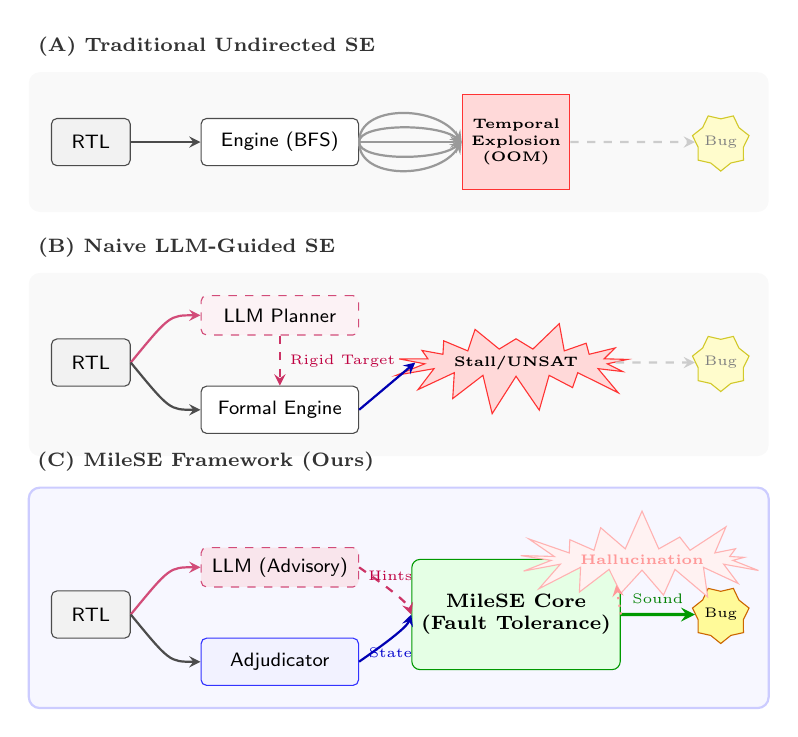
\begin{tikzpicture}[
        font=\sffamily\scriptsize,
        >=stealth,
        rtl/.style={draw=black!70, fill=gray!10, rounded corners=2pt, minimum height=6mm, minimum width=1.0cm, align=center},
        engine/.style={draw=black!70, fill=white, rounded corners=2pt, minimum height=6mm, minimum width=2.0cm, align=center},
        llm/.style={draw=purple!70, dashed, fill=purple!5, rounded corners=2pt, minimum height=5mm, minimum width=2.0cm, align=center},
        target/.style={draw=yellow!80!black, fill=yellow!20, star, star points=7, star point ratio=0.8, inner sep=1.5pt, align=center, font=\tiny},
        wall/.style={draw=red!80, fill=red!15, rectangle, minimum height=1.2cm, minimum width=6mm, align=center, font=\bfseries\tiny},
        explosion/.style={draw=red!80, fill=red!15, starburst, random starburst, inner sep=1pt, align=center, font=\bfseries\tiny},
        shield/.style={draw=green!60!black, fill=green!10, rounded corners=3pt, minimum height=1.4cm, minimum width=2.2cm, align=center, font=\bfseries\scriptsize},
        pathline/.style={->, thick, draw=blue!70!black},
        failpath/.style={->, thick, draw=black!40}
    ]

    % 背景层声明
    \pgfdeclarelayer{background}
    \pgfsetlayers{background,main}

    % ==========================================
    % (A) Traditional Undirected SE (BFS)
    % ==========================================
    \node[rtl] (rtl_a) at (0, 0) {RTL};
    \node[engine] (eng_a) at (2.4, 0) {Engine (BFS)};
    \node[wall] (wall_a) at (5.4, 0) {Temporal\\Explosion\\(OOM)};
    \node[target, text=gray] (bug_a) at (8, 0) {Bug};

    \draw[pathline, draw=black!70] (rtl_a) -- (eng_a);
    \foreach \y in {-0.4, -0.2, 0, 0.2, 0.4} {
        \draw[failpath] (eng_a.east) .. controls (3.4, \y*1.2) and (4.4, \y*1.2) .. (wall_a.west);
    }
    \draw[failpath, dashed, draw=black!20] (wall_a.east) -- (bug_a.west);


    % ==========================================
    % (B) Naive LLM-Guided SE
    % (Center shifted to Y = -2.8)
    % ==========================================
    \node[rtl] (rtl_b) at (0, -2.8) {RTL};
    
    \node[llm] (llm_b) at (2.4, -2.2) {LLM Planner};
    \node[engine] (eng_b) at (2.4, -3.4) {Formal Engine};
    
    \node[explosion] (gap_b) at (5.4, -2.8) {Stall/UNSAT};
    \node[target, text=gray] (bug_b) at (8, -2.8) {Bug};

    \draw[->, thick, draw=purple!70] (rtl_b.east) .. controls (1.0, -2.2) .. (llm_b.west);
    \draw[pathline, draw=black!70] (rtl_b.east) .. controls (1.0, -3.4) .. (eng_b.west);
    
    \draw[->, thick, draw=purple!80, dashed] (llm_b.south) -- node[right, font=\tiny, text=purple] {Rigid Target} (eng_b.north);
    \draw[pathline] (eng_b.east) -- (gap_b.west);
    \draw[failpath, dashed, draw=black!20] (gap_b.east) -- (bug_b.west);


    % ==========================================
    % (C) MileSE: Decoupled & Fault-Tolerant
    % (Center shifted to Y = -6.0)
    % ==========================================
    \node[rtl] (rtl_c) at (0, -6.0) {RTL};
    
    \node[llm, fill=purple!10] (llm_c) at (2.4, -5.4) {LLM (Advisory)};
    \node[engine, draw=blue!80, fill=blue!5] (eng_c) at (2.4, -6.6) {Adjudicator};
    
    \node[shield] (shield_c) at (5.4, -6.0) {MileSE Core\\(Fault Tolerance)};
    \node[target, draw=orange!80!black, fill=yellow!40, text=black] (bug_c) at (8, -6.0) {Bug};

    \draw[->, thick, draw=purple!70] (rtl_c.east) .. controls (1.0, -5.4) .. (llm_c.west);
    \draw[pathline, draw=black!70] (rtl_c.east) .. controls (1.0, -6.6) .. (eng_c.west);
    
    \draw[->, thick, draw=purple!80, dashed] (llm_c.east) .. controls (3.4, -5.4) and (4.0, -5.8) .. (shield_c.west) node[pos=0.6, above, font=\tiny, text=purple] {Hints};
    \draw[pathline] (eng_c.east) .. controls (3.4, -6.6) and (4.0, -6.2) .. (shield_c.west) node[pos=0.6, below, font=\tiny, text=blue!80!black] {State};

    \draw[pathline, line width=1.2pt, draw=green!60!black] (shield_c.east) -- node[above, font=\tiny, text=green!50!black] {Sound} (bug_c.west);

    \node[explosion, draw=red!30, fill=red!5, text=red!40, scale=1] (fake_gap) at (7, -5.3) {Hallucination};
    \draw[->, thick, dotted, draw=red!40] (shield_c.east) -- (fake_gap.south west);


    % ==========================================
    % Background Boxes with Auto-Aligned Labels
    % ==========================================
    \begin{pgfonlayer}{background}
        \node[fill=gray!5, rounded corners=4pt, fit=(rtl_a)(eng_a)(wall_a)(bug_a), inner sep=8pt,
              label={[anchor=south west, font=\bfseries\scriptsize, text=black!80, yshift=2pt]north west:(A) Traditional Undirected SE}] {};
              
        \node[fill=gray!5, rounded corners=4pt, fit=(rtl_b)(llm_b)(eng_b)(gap_b)(bug_b), inner sep=8pt,
              label={[anchor=south west, font=\bfseries\scriptsize, text=black!80, yshift=2pt]north west:(B) Naive LLM-Guided SE}] {};
              
        \node[fill=blue!3, draw=blue!20, thick, rounded corners=4pt, fit=(rtl_c)(llm_c)(eng_c)(shield_c)(bug_c)(fake_gap), inner sep=8pt,
              label={[anchor=south west, font=\bfseries\scriptsize, text=black!80, yshift=2pt]north west:(C) MileSE Framework (Ours)}] {};
    \end{pgfonlayer}

    \end{tikzpicture}%
    }
    \caption{Comparison of multi-cycle symbolic execution paradigms. (A) Undirected search suffers from temporal path explosion. (B) Naive LLM guidance faces a STall/UNSAT. (C) \textbf{MileSE} strictly decouples advisory hints from formal adjudication, utilizing fault tolerance to bypass hallucinations.}
    \label{fig:teaser}
\end{figure}

This paper introduces \textbf{MileSE}, a milestone-guided symbolic execution framework designed to tolerate these inaccuracies. As illustrated in Fig. \ref{fig:teaser}, MileSE relies on a strict architectural decoupling: LLM milestones merely suggest promising directions, while the underlying solver retains full control over proving path feasibility and confirming violations.

To make this guidance robust against real-world hardware complexities, MileSE goes beyond a simple priority queue. It employs a \textit{Dual-Track Scoring} mechanism to sustain directed progress during sparse milestone intervals. Additionally, MileSE relies on system-level fault-tolerance features, including \textit{sliding-window lookahead} and \textit{eager target evaluation}, to safely bypass LLM hallucinations. As a result, the framework significantly compresses the multi-cycle state space without introducing any false negatives.

In summary, this paper makes the following key contributions:
\begin{itemize}
    \item We identify \textit{temporal path explosion} as the primary scaling bottleneck in multi-cycle RTL symbolic execution, demonstrating the fundamental limitations of undirected search strategies.
    \item We propose a robust milestone-guided architecture that strictly decouples probabilistic LLM hints from deterministic formal checking, preserving absolute verification soundness.
    \item We design and implement MileSE with system-level fault-tolerance mechanisms—specifically \textit{Dual-Track Scoring}, \textit{Sliding-Window Lookahead}, and \textit{Eager Target Evaluation}—to robustly navigate sparse milestone intervals and safely bypass LLM hallucinations.
    \item We evaluate MileSE on complex sequential RTL properties. Experimental results show that MileSE drastically reduces execution time, memory footprint, and SMT query counts compared to state-of-the-art engines, strictly guaranteeing zero false negatives.
\end{itemize}



\section{Background and Motivation}
\label{sec:background}

\subsection{Hardware Symbolic Execution}
An RTL symbolic executor maintains states of the form $(stmt,\sigma,\pi)$, where $stmt$ is the next statement, $\sigma$ maps RTL objects to symbolic expressions, and $\pi$ is the path condition. When a conditional branch is encountered, the executor forks states and extends $\pi$ with the branch predicate or its negation. When an assertion can be violated under $\pi$, the solver returns a satisfying model that can serve as a counterexample.

RTL execution adds cycle-level structure to this model. Blocking assignments update the current symbolic store immediately, while non-blocking assignments are buffered and committed at a clock boundary. Registers persist across cycles, primary inputs may be refreshed with fresh symbolic values, and combinational logic must be reevaluated after state changes. These semantics make direct RTL symbolic execution expressive, but they also create repeated frontier-selection decisions across cycles.

The search problem studied here is therefore not only whether one branch inside an always block is feasible. It is whether a feasible state at the end of a cycle deserves further exploration before many other feasible states. This distinction matters for long-trigger properties, where most legal continuations do not make progress toward the vulnerable state.


\begin{figure}[h!]
\begin{framed}
\begin{lstlisting}[caption={Accumulator used to illustrate temporal search difficulty.},label={lst:toy_acc}]
module accumulator (
    input  CLK,
    input  RST,
    input  valid,
    output reg [31:0] out
);
    initial out = 0;
    always @(posedge CLK) begin
        if (RST) begin
            out <= 0;
        end else if (valid) begin
            out <= out + 1;
        end
        if (!RST) begin
            assert (out <= 3);
        end
    end
endmodule
\end{lstlisting}
\end{framed}
\caption{Motivating Verilog Code}
\label{fig:verilog-fig}

\end{figure}

\subsection{Large Language Models}
Large Language Models (LLMs) have seen widespread adoption across electronic design automation (EDA) tasks [11]--[13]. Recent frameworks leverage LLM reasoning to automate HDL code generation, employing techniques ranging from advanced prompt engineering and Monte Carlo Tree Search (MCTS) [13]--[17] to dedicated platforms like ChipGPT [18]. In the verification domain, LLMs have also proven effective at analyzing hardware semantics to generate security assertions and identify common vulnerabilities [19], [20].

However, because foundational models are pre-trained primarily on general-purpose text corpora, they frequently suffer from domain misalignment when applied to specialized hardware contexts [10], [21]. Since training a massive LLM from scratch for RTL tasks is computationally prohibitive, parameter-efficient fine-tuning (PEFT) has become a highly accessible alternative [22]. Techniques such as Low-Rank Adaptation (LoRA) [8] allow engineers to update only a small fraction of the model's weights, effectively adapting open-source LLMs to specific downstream EDA applications.

MileSE applies these fine-tuned models to address the temporal path explosion in symbolic execution. Instead of generating code or assertions, the LLM serves as a high-level planner. By analyzing the RTL design and the target property, it extracts a sequence of intermediate \textit{milestones}. To concretely illustrate how these milestones guide the formal engine---and why they must be treated as heuristics rather than rigid constraints---we introduce a motivating RTL example below.

\subsection{Motivating Example: The Temporal Bottleneck}

\begin{figure}[htbp]
    \centering
    \resizebox{\linewidth}{!}{%
    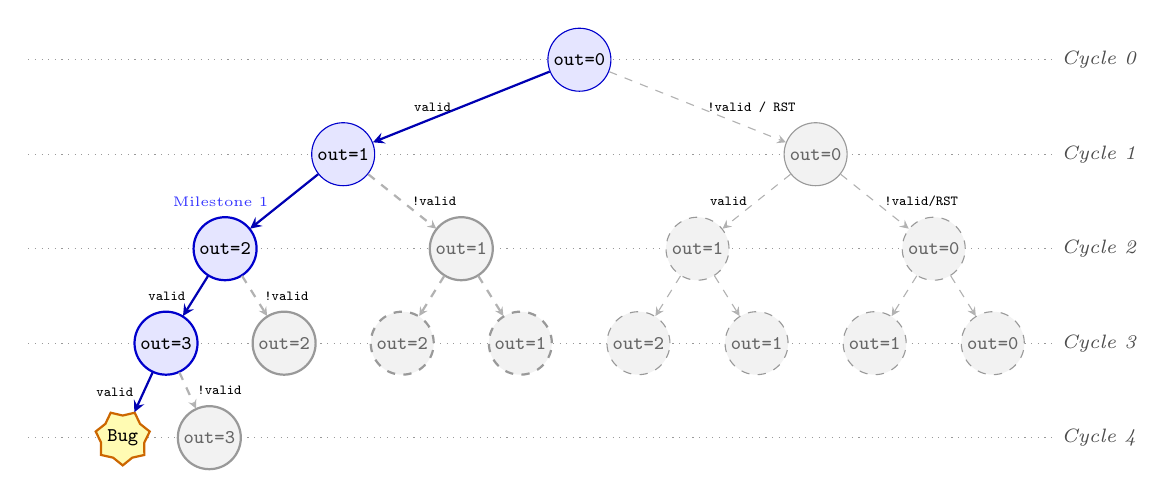
\begin{tikzpicture}[
        >=stealth,
        font=\sffamily\scriptsize,
        level distance=1.2cm,
        % 精准分配每一层的子节点间距，严格防止重叠
        level 1/.style={sibling distance=6.0cm},
        level 2/.style={sibling distance=3.0cm},
        level 3/.style={sibling distance=1.5cm},
        level 4/.style={sibling distance=1.1cm},
        % 节点样式定义
        milestone/.style={draw=blue!80!black, fill=blue!10, circle, minimum size=8mm, inner sep=1pt, font=\bfseries\scriptsize},
        wasted/.style={draw=black!40, fill=gray!10, circle, minimum size=8mm, inner sep=1pt, text=black!60},
        target/.style={draw=orange!80!black, fill=yellow!30, star, star points=7, star point ratio=0.8, inner sep=1.5pt},
        % 连线样式定义
        goodpath/.style={->, thick, draw=blue!70!black},
        badpath/.style={->, draw=black!30, dashed},
        % 标签样式
        cyclelabel/.style={font=\itshape\scriptsize, text=black!70, anchor=west}
    ]

    % 定义树的结构
    \node[milestone] (root) {\texttt{out=0}}
        child {
            node[milestone] (c1_good) {\texttt{out=1}}
            child {
                node[milestone] (c2_good) {\texttt{out=2}}
                child {
                    node[milestone] (c3_good) {\texttt{out=3}}
                    child {
                        node[target] (bug) {\texttt{Bug}}
                        edge from parent[goodpath] node[left, font=\tiny] {\texttt{valid}}
                    }
                    child {
                        node[wasted] (c4_bad) {\texttt{out=3}}
                        edge from parent[badpath] node[right, font=\tiny] {\texttt{!valid}}
                    }
                    edge from parent[goodpath] node[left, font=\tiny] {\texttt{valid}}
                }
                child {
                    node[wasted] (c3_bad1) {\texttt{out=2}}
                    edge from parent[badpath] node[right, font=\tiny] {\texttt{!valid}}
                }
                edge from parent[goodpath] node[left=2pt, font=\tiny, text=blue!80] {Milestone 1}
            }
            child {
                node[wasted] (c2_bad1) {\texttt{out=1}}
                child {
                    node[wasted] (c3_bad2) {\texttt{out=2}}
                    edge from parent[badpath]
                }
                child {
                    node[wasted] (c3_bad3) {\texttt{out=1}}
                    edge from parent[badpath]
                }
                edge from parent[badpath] node[right, font=\tiny] {\texttt{!valid}}
            }
            edge from parent[goodpath] node[left, font=\tiny] {\texttt{valid}}
        }
        child {
            node[wasted] (c1_bad) {\texttt{out=0}}
            child {
                node[wasted] (c2_bad2) {\texttt{out=1}}
                child {
                    node[wasted] (c3_bad4) {\texttt{out=2}}
                    edge from parent[badpath]
                }
                child {
                    node[wasted] (c3_bad5) {\texttt{out=1}}
                    edge from parent[badpath]
                }
                edge from parent[badpath] node[left, font=\tiny] {\texttt{valid}}
            }
            child {
                node[wasted] (c2_bad3) {\texttt{out=0}}
                child {
                    node[wasted] (c3_bad6) {\texttt{out=1}}
                    edge from parent[badpath]
                }
                child {
                    node[wasted] (c3_bad7) {\texttt{out=0}}
                    edge from parent[badpath]
                }
                edge from parent[badpath] node[right, font=\tiny] {\texttt{!valid\\/RST}}
            }
            edge from parent[badpath] node[right, font=\tiny] {\texttt{!valid / RST}}
        };

    % 添加周期标签和横向虚线背景（同步调整了线的宽度以适应新树宽）
    \begin{pgfonlayer}{background}
        \draw[dotted, draw=black!40] (-7.0, 0) -- (6.0, 0) node[cyclelabel] {Cycle 0};
        \draw[dotted, draw=black!40] (-7.0, -1.2) -- (6.0, -1.2) node[cyclelabel] {Cycle 1};
        \draw[dotted, draw=black!40] (-7.0, -2.4) -- (6.0, -2.4) node[cyclelabel] {Cycle 2};
        \draw[dotted, draw=black!40] (-7.0, -3.6) -- (6.0, -3.6) node[cyclelabel] {Cycle 3};
        \draw[dotted, draw=black!40] (-7.0, -4.8) -- (6.0, -4.8) node[cyclelabel] {Cycle 4};
    \end{pgfonlayer}

    \end{tikzpicture}%
    }
    \caption{Symbolic execution tree for the accumulator (Listing \ref{lst:toy_acc}). A standard BFS blindly expands all semantically legal branches (gray nodes), leading to temporal explosion. MileSE leverages intermediate milestones (e.g., \texttt{out==1}, \texttt{out==2}) to strictly prioritize the single path (blue nodes) leading to the assertion violation.}
    \label{fig:sym_tree}
\end{figure}

To illustrate why multi-cycle search is challenging, how milestones help, and what can go wrong, consider the accumulator in Fig.~\ref{fig:verilog-fig} and its corresponding symbolic execution tree in Fig.~\ref{fig:sym_tree}.

%\textbf{Temporal Path Explosion.} 
The assertion violation requires the counter to strictly exceed 3, which demands at least four clock cycles where \texttt{RST} is low and \texttt{valid} is high. As illustrated by the exponentially expanding gray nodes in Fig.~\ref{fig:sym_tree}, a blind symbolic executor utilizing Breadth-First Search (BFS) will fork at every cycle on the \texttt{RST} and \texttt{valid} branches. It wastes massive computational resources exploring semantically legal alternatives---such as continuously asserting reset (\texttt{out <= 0}) or stalling the counter (\texttt{valid == 0})---that never move toward the vulnerable state. 

%\textbf{The Power of Milestones.} 
For this example, useful progress is easy to describe: \texttt{out == 1} $\rightarrow$ \texttt{out == 2} $\rightarrow$ \texttt{out == 3}. As highlighted by the targeted blue path in Fig.~\ref{fig:sym_tree}, if an LLM provides these intermediate conditions as milestones, the engine can prioritize states that satisfy them. Crucially, these milestones provide only a \textit{weak notion of temporal progress}; they are not proof obligations. Instead of permanently injecting them into the path condition, the engine checks whether the current path satisfies the next milestone. If so, the state receives a better priority score and is explored earlier. This transforms a computationally expensive, undirected $2^N$ exploration into a highly targeted progression toward the bug, making the search highly directed without altering the strict formal semantics of the underlying executor.

%\textbf{LLM Hallucinations and Search Stalls.} 
However, naive milestone guidance is inherently unreliable. Since LLMs are probabilistic, they frequently generate flawed milestones. For instance, an LLM might hallucinate an incorrect signal name (e.g., \texttt{rst\_n == 0} instead of \texttt{RST}), propose a physically impossible state transition (e.g., \texttt{out} jumping directly from 0 to 2 in a single cycle), or suggest a condition mathematically inconsistent with the current path constraint. If the formal engine rigidly enforces these flawed milestones, the SMT solver will return UNSAT, causing the search to hit a dead end and fail to find the bug. 

These failure modes fundamentally shape the design of MileSE: the system must leverage the heuristic power of LLM milestones while systematically tolerating their inaccuracies to preserve formal soundness.

\section{MileSE System Architecture}
\label{sec:architecture}

\begin{figure}[t]
    \centering
    \resizebox{\linewidth}{!}{%
    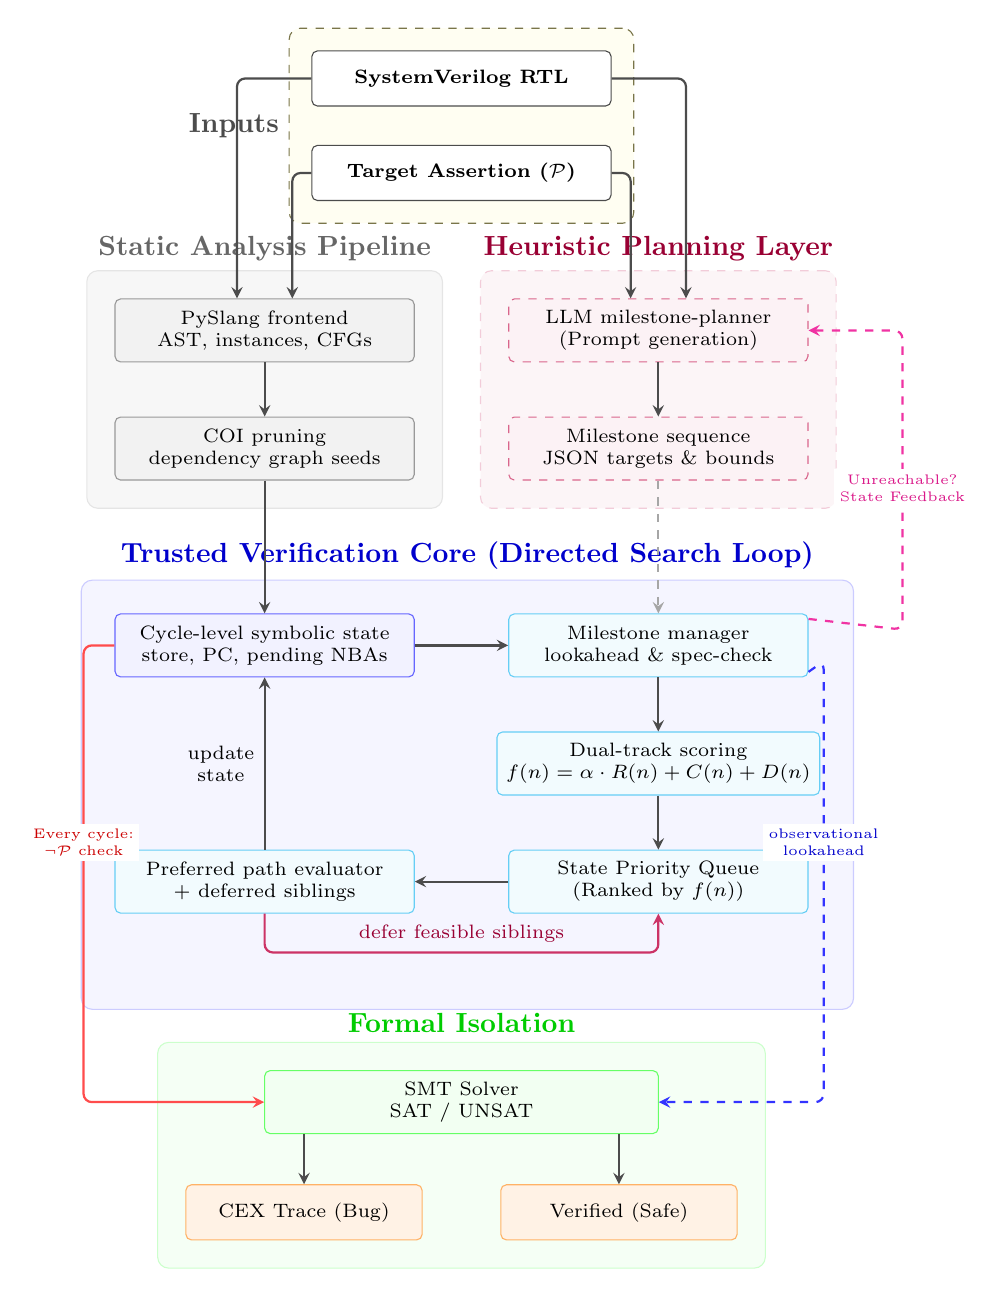
\begin{tikzpicture}
        % 声明背景层
        \pgfdeclarelayer{background}
        \pgfsetlayers{background,main}

        % 全局样式定义
        \tikzset{
            font=\scriptsize,
            >=stealth,
            inputbox/.style={draw=black!70, fill=white, rectangle, rounded corners=2pt, minimum height=7mm, minimum width=3.8cm, align=center, font=\bfseries\scriptsize},
            block/.style={draw=gray!80, fill=gray!10, rectangle, rounded corners=2pt, minimum height=8mm, minimum width=3.8cm, align=center},
            advisory/.style={draw=purple!60, dashed, fill=purple!5, rectangle, rounded corners=2pt, minimum height=8mm, minimum width=3.8cm, align=center},
            trusted/.style={draw=blue!60, fill=blue!5, rectangle, rounded corners=2pt, minimum height=8mm, minimum width=3.8cm, align=center},
            guard/.style={draw=cyan!60, fill=cyan!5, rectangle, rounded corners=2pt, minimum height=8mm, minimum width=3.8cm, align=center},
            solver/.style={draw=green!60, fill=green!5, rectangle, rounded corners=2pt, minimum height=8mm, minimum width=5cm, align=center},
            output/.style={draw=orange!60, fill=orange!10, rectangle, rounded corners=2pt, minimum height=7mm, minimum width=3cm, align=center},
            flow/.style={->, thick, draw=black!70, rounded corners=3pt},
            softflow/.style={->, thick, dashed, draw=gray!70, rounded corners=3pt}
        }

        % ================= 1. Top Level Inputs =================
        \node[inputbox] (rtl) at (0, 10.2) {SystemVerilog RTL};
        \node[inputbox] (assert) at (0, 9) {Target Assertion ($\mathcal{P}$)};


        % ================= 2. Parallel Pipelines (Static & LLM) =================
        % Left side: Static Analysis
        \node[block] (frontend) at (-2.5, 7) {PySlang frontend\\AST, instances, CFGs};
        \node[block] (coi) at (-2.5, 5.5) {COI pruning\\dependency graph seeds};

        % Right side: Heuristic Planning Layer
        \node[advisory] (planner) at (2.5, 7) {LLM milestone-planner\\(Prompt generation)};
        \node[advisory] (milestones) at (2.5, 5.5) {Milestone sequence\\JSON targets \& bounds};


        % ================= 3. Dynamic Core Loop =================
        \node[trusted] (state) at (-2.5, 3) {Cycle-level symbolic state\\store, PC, pending NBAs};
        \node[guard] (manager) at (2.5, 3) {Milestone manager\\lookahead \& spec-check};
        
        \node[guard] (score) at (2.5, 1.5) {Dual-track scoring\\$f(n)=\alpha \cdot R(n)+C(n)+D(n)$};
        
        % 修改点：去除 min-heap 和 WorkItems，拔高为状态优先级队列
        \node[guard] (queue) at (2.5, 0) {State Priority Queue\\(Ranked by $f(n)$)};
        \node[guard] (fork) at (-2.5, 0) {Preferred path evaluator\\+ deferred siblings};
        
        % 占位符：扩充 Core Loop 底部包围盒
        \coordinate (dummy_bottom) at (0, -1.2);


        % ================= 4. Solver & Outputs =================
        \node[solver] (z3) at (0, -2.8) {SMT Solver\\SAT / UNSAT};
        \node[output] (cex) at (-2, -4.2) {CEX Trace (Bug)};
        \node[output] (safe) at (2, -4.2) {Verified (Safe)};


        % ================= Hierarchical Backgrounds =================
        \begin{pgfonlayer}{background}
            % Inputs Box
            \node[fill=yellow!5, draw=yellow!40!black, dashed, rounded corners=4pt, fit=(rtl)(assert), inner sep=8pt, label={[font=\bfseries, text=black!70]left:Inputs}] {};

            % Static Analysis Box (Left)
            \node[fill=gray!6, draw=gray!20, rounded corners=4pt, fit=(frontend)(coi), inner sep=10pt, label={[font=\bfseries, text=gray!80!black]above:Static Analysis Pipeline}] {};

            % Heuristic Planning Box (Right)
            \node[fill=purple!4, draw=purple!20, dashed, rounded corners=4pt, fit=(planner)(milestones), inner sep=10pt, label={[font=\bfseries, text=purple!80!black]above:Heuristic Planning Layer}] {};

            % Dynamic Core Box (Center)
            \node[fill=blue!4, draw=blue!20, rounded corners=4pt, fit=(state)(manager)(score)(queue)(fork)(dummy_bottom), inner sep=12pt, label={[font=\bfseries, text=blue!80!black]above:Trusted Verification Core (Directed Search Loop)}] {};

            % Formal Adjudication Box (Bottom)
            \node[fill=green!4, draw=green!20, rounded corners=4pt, fit=(z3)(cex)(safe), inner sep=10pt, label={[font=\bfseries, text=green!80!black]above:Formal Isolation}] {};
        \end{pgfonlayer}


        % ================= Routing / Connections =================
        % 1. Input Distribution (Perfect Nested Routing - No Crossings!)
        % RTL flows to the outer edges of Frontend and Planner
        \draw[flow] (rtl.west) -| ([xshift=-10pt]frontend.north);
        \draw[flow] (rtl.east) -| ([xshift=10pt]planner.north);
        
        % Assert flows to the inner edges of Frontend and Planner
        \draw[flow] (assert.west) -| ([xshift=10pt]frontend.north);
        \draw[flow] (assert.east) -| ([xshift=-10pt]planner.north);

        % 2. Parallel Pipelines Internal Flow
        \draw[flow] (frontend) -- (coi);
        \draw[flow] (planner) -- (milestones);

        % 3. Bridge into Core Loop
        \draw[flow] (coi) -- (state);
        \draw[softflow] (milestones) -- (manager);

        % 4. The Core Execution Loop (Counter-Clockwise Rectangle)
        \draw[flow] (state) -- (manager);
        \draw[flow] (manager) -- (score);
        \draw[flow] (score) -- (queue);
        \draw[flow] (queue) -- (fork);
        \draw[flow] (fork) -- (state) node[midway, left, align=center] {update\\state};

        % 5. Sibling Feedback
        \draw[flow, draw=purple!80] (fork.south) -- (-2.5, -0.9) -- (2.5, -0.9) -- (queue.south);
        \node[above, text=purple!80!black] at (0, -0.9) {defer feasible siblings};

        % 6. Z3 Connectors (Wraparound Side Corridors)
        %   - Left Corridor: Eager Target Evaluation
        \draw[flow, draw=red!70, thick] (state.west) -- (-4.8, 3) -- (-4.8, -2.8) -- (z3.west);
        \node[align=center, fill=white, inner sep=2pt, text=red!80!black, font=\tiny] at (-4.8, 0.5) {Every cycle:\\$\neg \mathcal{P}$ check};

        %   - Right Corridor: Observational Lookahead
        \draw[softflow, draw=blue!80, thick] (manager.-10) -- (4.6, 2.8) -- (4.6, -2.8) -- (z3.east);
        \node[align=center, fill=white, inner sep=2pt, text=blue!80!black, font=\tiny] at (4.6, 0.5) {observational\\lookahead};

        % 7. Milestone Correction Feedback Loop
        \draw[flow, dashed, draw=magenta!80, thick] (manager.10) -- (5.6, 3.2) -- (5.6, 7) -- (planner.east);
        \node[align=center, fill=white, inner sep=2pt, text=magenta!90!black, font=\tiny] at (5.6, 5) {Unreachable?\\State Feedback};

        % 8. Outputs
        \draw[flow] (z3.south -| cex.north) -- (cex.north);
        \draw[flow] (z3.south -| safe.north) -- (safe.north);

    \end{tikzpicture}%
    }
    \caption{Vertical architecture of MileSE. The formal context and LLM-generated milestones are processed through two parallel pipelines (Static Analysis and Heuristic Planning). These streams converge in the central directed search loop. To ensure system liveness, if a milestone is proven unreachable, the manager uses the feedback corridor (magenta) to prompt the LLM for dynamic re-planning. Formal soundness is strictly isolated via independent SMT side-channel checks.}
    \label{fig:milese_overview}
\end{figure}
\subsection{Architecture Overview}
As illustrated in Fig. \ref{fig:milese_overview}, the architecture of MileSE is organized around a strict formal boundary, processing inputs through two parallel pipelines. On the left, the \textbf{Static Analysis Pipeline} parses the SystemVerilog design and prunes irrelevant logic to establish a deterministic execution context. Concurrently on the right, the \textbf{Heuristic Planning Layer} employs an LLM to analyze the target assertion and generate a sequence of cycle-bounded milestones.

These two streams converge in the central \textbf{Directed Search Loop}. Here, the engine uses the milestones as flexible milestones to prioritize exploration, rather than treating them as rigid constraints. To prevent the search from hitting a dead end, a feedback loop (magenta dashed line) actively monitors the execution. If a milestone turns out to be unreachable, the manager immediately feeds the current state back to the LLM to generate a new, valid plan.

Crucially, as shown at the bottom of the architecture, all semantic validation—including branch feasibility and final assertion checking—is structurally isolated and offloaded to an independent SMT solver. This design guarantees that the LLM solely guides the search trajectory, while the formal engine retains absolute authority over bug discovery and verification soundness.

\subsection{Frontend Analysis and Milestone Generation}
Before the dynamic search begins, MileSE prepares the verification context through a deterministic \textbf{Static Analysis Pipeline} and a \textbf{Heuristic Planning Layer} powered by an LLM.

\subsubsection{RTL Elaboration and COI Pruning}
The framework leverages a PySlang frontend to elaborate the RTL, extract procedural control-flow graphs (CFGs), record combinational dependencies, and build a cycle-accurate symbolic execution context. As an orthogonal optimization, MileSE performs Cone-of-Influence (COI) pruning. Using the target assertion expressions and milestone-related signals as seeds, the engine statically removes hardware logic that cannot affect the property, significantly reducing the amount of RTL the executor must carry.

\subsubsection{LLM Milestone-Planning and Context Engineering}
Operating in parallel to the formal setup, a fine-tuned LLM analyzes the design to generate a sequence of intermediate milestones. To ensure the LLM's output is both syntactically parsable and semantically grounded, MileSE employs a highly structured prompt engineering pipeline rather than feeding raw source code. 

The prompt context is meticulously constructed using three curated inputs: (1) the \textit{Target Assertion}, which defines the final vulnerability; (2) the \textit{Procedural CFGs}, which provide the model with explicit spatial and temporal control-flow dependencies; and (3) the \textit{COI-pruned RTL code}, which drastically reduces the token overhead by filtering out irrelevant hardware logic, ensuring the design fits well within the LLM's context window.

To prevent formatting hallucinations and enable automated parsing by the downstream engine, the LLM is strictly instructed to output the macro-plan matching a standardized JSON template. As shown in Listing \ref{lst:json_template}, each milestone must explicitly declare its expected clock cycle budget (\texttt{cycle\_bound}) and a mathematically verifiable RTL expression (\texttt{condition}). 

\begin{lstlisting}[language=json, aboveskip=1.5em, belowskip=1em, caption={Standardized JSON template for LLM milestone generation.}, label={lst:json_template}, basicstyle=\ttfamily\scriptsize, frame=single, numbers=left, xleftmargin=2em]
{
  "milestones": [
    {
      "step": 1,
      "intent": "Release system reset and wait for initialization",
      "cycle_bound": 2,
      "condition": "RST == 1'b0"
    },
    {
      "step": 2,
      "intent": "Trigger the valid signal to start accumulation",
      "cycle_bound": 5,
      "condition": "valid == 1'b1 && out == 32'd1"
    }
  ]
}
\end{lstlisting}

This context-aware, template-driven generation transforms a deep, complex verification target into localized, cycle-bounded RTL sub-goals, providing the formal engine with strict spatial and temporal scheduling guidance.


\subsection{Dual-Track Directed Search}
To prevent the execution from degenerating into undirected Breadth-First Search (BFS) during sparse multi-cycle intervals between milestones, MileSE introduces a Dual-Track Scoring strategy. This mechanism elegantly fuses high-level heuristic planning from the LLM with low-level structural gradients from the formal engine. Each symbolic state $n$ in the priority queue is ranked by a comprehensive scheduling priority $f(n)$:
\begin{equation}
    f(n) = \alpha \cdot R(n) + C(n) + \min(D(n), D_{\max})
\end{equation}
where a lower score indicates a higher execution priority.

\textbf{Global Milestone Track.} $R(n)$ tracks the number of milestones left to reach, and $C(n)$ counts the elapsed clock cycles. A large weight $\alpha$ ensures the engine strongly prioritizes states that have completed more milestones. If multiple states share the same milestone progress, $C(n)$ acts as a tie-breaker, naturally favoring the path that took fewer cycles.

\textbf{Local Gradient Track.} When milestone progress stalls over multiple cycles, the distance metric $D(n)$ breaks the tie. MileSE utilizes a SMT solver to calculate the numerical difference between the current signal value and the target (e.g., $\Delta = |v_{\text{current}} - v_{\text{target}}|$). This difference acts as a local gradient, guiding the search step-by-step toward the next milestone.

\textbf{Preferred-Path Execution.} To translate this priority into execution efficiency, MileSE adopts a highly selective branching strategy. When encountering a conditional AST branch, the engine evaluates only the "preferred path" dictated by $D(n)$. Alternative feasible sibling branches are encapsulated as lightweight state snapshots and deferred to the priority queue (as shown by the purple feedback loop in Fig. \ref{fig:milese_overview}), ensuring heavy SMT resources are exclusively committed to the milestone trajectory.


\subsection{Mitigating LLM Hallucinations}
A naive integration of LLMs causes formal engines to hit dead ends when milestones contain hallucinated signals or temporally skipped states. MileSE guarantees absolute verification soundness and system liveness through four fault-tolerant mechanisms.

\subsubsection{Observational Checking and Bounded Deprioritization}
Milestones are treated exclusively as \textit{observational hints}. When checking if a state satisfies a milestone $M_i$, the manager issues speculative SMT queries using context scopes. If the milestone is unsatisfiable or references nonexistent identifiers, the constraint is safely discarded without polluting the symbolic path condition. Furthermore, the engine uses the \texttt{expected\_cycles} metric $k$ as a flexible timeout threshold. By introducing a constant tolerance margin $\Delta$, if a state fails to make milestone progress after $k + \Delta$ cycles, its execution priority is heavily reduced. This allowance compensates for the LLM's imprecise cycle estimations while still preventing the solver from wasting computational resources on dead-end paths.

\subsubsection{Sliding-Window Lookahead}
To counter temporal mismatch (e.g., the state transitions from $0$ to $2$, bypassing milestone $1$), MileSE employs a Sliding-Window Lookahead. If the immediate milestone $M_{i}$ is unresolvable, the engine non-blockingly evaluates $M_{i+1}$. If the future milestone evaluates to \texttt{SAT}, the engine shifts its focus and drops the hallucinated intermediate milestones.

\subsubsection{Dynamic Re-Planning Feedback Loop}
When the sliding-window mechanism confirms that a milestone is structurally unreachable from the current promising frontier, MileSE leverages the state feedback loop (highlighted by the magenta dashed line in Fig. \ref{fig:milese_overview}). The Milestone Manager extracts verifiable state conditions from Z3 and feeds them back to the LLM. The LLM then issues a revised, locally reachable sequence of milestones, ensuring overall system liveness.

\subsubsection{Eager Target Evaluation}
While intermediate milestones guide the heuristic search, they cannot be trusted to validate the final vulnerability. To guarantee zero false negatives, MileSE implements Eager Target Evaluation. At every clock cycle transition, as indicated by the red eager-check corridor in Fig. \ref{fig:milese_overview}, the engine speculatively injects the negated global assertion condition ($\neg \mathcal{P}_{\text{target}}$) into the solver. If this query returns \texttt{SAT}, MileSE instantly terminates the search and reconstructs a mathematically proven counterexample trace.

\section{Implementation and Evaluation}
\label{sec:evaluation}

\section{Experimental Evaluation}
\label{sec:evaluation}

Our experimental evaluation is designed to answer one central research question: \textit{Does milestone-guided scheduling effectively reduce temporal path explosion on deep sequential RTL properties while strictly preserving formal verification soundness (zero false negatives)?} 

\subsection{Implementation Details}
We implemented the MileSE framework as a custom Python-based symbolic execution engine. The frontend leverages \textbf{PySlang} for rigorous SystemVerilog parsing, elaboration, and cycle-accurate Abstract Syntax Tree (AST) generation. The deterministic formal checking is powered by the \textbf{Z3 SMT solver}. MileSE seamlessly integrates the proposed dual-track priority queue and system-level fault-tolerance mechanisms. To ensure optimal execution semantics, the engine dynamically constructs procedural Control Flow Graphs (CFGs) and applies Cone-of-Influence (COI) pruning directly on the AST prior to Z3 query formulation. The LLM milestone generation is handled via API calls to a fine-tuned instruction model.

\subsection{Experimental Setup and Baselines}
To evaluate the effectiveness and scalability of MileSE, we conduct experiments on representative multi-cycle RTL designs, specifically focusing on HACK@DAC hardware-security benchmarks and OR1200-derived assertion suites. We compare our approach against the following baselines:
\begin{itemize}
    \item \textbf{Baseline (Undirected SE):} A standard, unguided symbolic execution engine utilizing a Breadth-First Search (BFS) policy. It shares the exact same PySlang frontend and Z3 backend but lacks LLM milestone prioritization.
    \item \textbf{MileSE (no-COI):} Our milestone-directed search framework with all fault-tolerance mechanisms enabled, but without structural Cone-of-Influence pruning.
    \item \textbf{MileSE (Full):} The complete proposed framework, combining LLM milestone guidance, fault tolerance, and COI pruning.
\end{itemize}

To rigorously quantify the verification overhead and bug-finding capabilities, we measure the following primary metrics across all configurations: total execution runtime, time-to-first-violation, total number of explored symbolic states, simulated clock cycles, and final solver-validated violations. 


% ==========================================
% USER FILL IN: Section 6.3 - Main Results
% ==========================================
\subsection{Overall Verification Performance}
\label{subsec:eval_overall}

% [TODO: Insert your main results table here]
\begin{table}[htbp]
    \centering
    \caption{Overall performance comparison between Baseline, MileSE (no-COI), and MileSE (Full) across various benchmarks. (T.O. = Time Out)}
    \label{tab:main_results}
    \resizebox{\linewidth}{!}{%
    \begin{tabular}{l c c c c c c}
        \toprule
        \textbf{Benchmark} & \textbf{Metric} & \textbf{Baseline (BFS)} & \textbf{MileSE (no-COI)} & \textbf{MileSE (Full)} & \textbf{Speedup} \\
        \midrule
        % Example Row:
        % Hack@DAC-1 & Runtime (s) & T.O. (>7200) & 145.2 & 112.5 & >64x \\
        [TODO: Data] & & & & & \\
        \bottomrule
    \end{tabular}
    }
\end{table}

As shown in Table \ref{tab:main_results}, the baseline undirected engine suffers from severe temporal path explosion, resulting in timeouts (T.O.) on deeply sequential properties. In contrast, MileSE... 
% [TODO: Write 1-2 paragraphs analyzing the table. Emphasize how the milestone guidance prevents BFS explosion, and how COI further reduces the state payload.]


% ==========================================
% USER FILL IN: Section 6.4 - Ablation Study
% ==========================================
\subsection{Ablation Study: System-Level Mechanisms}
\label{subsec:eval_ablation}
Beyond the end-to-end comparisons, we conduct an ablation study to isolate the impact of individual system-level mechanisms, specifically evaluating the contributions of the dual-track scoring

\section{Related Work}
\label{sec:related}
RTL symbolic execution research has attacked path explosion by exploiting hardware structure. Structural decomposition, shared processing of independent procedural blocks, and solver-query reuse reduce redundant work inside or across cycle-level RTL components. MileSE is complementary to that line of work. It assumes such reductions are useful, but focuses on the remaining temporal question of which feasible post-cycle states deserve priority.

Directed symbolic execution and concolic testing use targets, program context, or path information to reach interesting behaviors faster. MileSE follows the same broad intuition but applies it to direct RTL execution and treats milestones as solver-checked observations over the current symbolic store. The method is not semantic pruning of all irrelevant states; it is priority scheduling with conservative local pruning.

Recent LLM-assisted verification and symbolic-execution systems show that language models can generate tests, guide paths, or provide high-level decomposition. MileSE uses this capability narrowly. A model may propose milestone conditions, but the formal engine parses them, checks whether signals resolve, asks the solver whether they are feasible, and validates assertion violations. This separation is the main distinction between MileSE and approaches where the generated text or test itself carries more of the verification burden.

\section{Conclusion}
\label{sec:conclusion}
MileSE addresses a temporal bottleneck in multi-cycle RTL symbolic execution: many feasible states are legal, but few move toward a deep target property. The framework uses milestones to prioritize the search queue while leaving feasibility and violation checks under solver control. Its implementation combines compound milestone parsing, bounded local exploration, conservative recovery, cycle-aware RTL semantics, targeted combinational reevaluation, and optional COI pruning. The next step is to complete the planned quantitative evaluation so the paper can report how much this solver-owned guidance reduces wasted exploration on representative sequential RTL properties.

\section*{Acknowledgment}
Acknowledgment text will be finalized in the camera-ready version.

\bibliographystyle{IEEEtran}
\bibliography{ref}

\end{document}
